\subsection[Non-isothermal two-phase flow]{Non-isothermal two-phase flow of compressible fluids (H$^2$T-process)}

\subsubsection*{Intro}

In this test case, compressible two-phase flow of real gases is considered. The transport properties of the fluids are determined by accurate constitutive correlations (see sections \ref{sec-viscosity} and \ref{sec-thermal-conductivity}). With the chosen conditions of pressure and temperature, the gases are in a supercritical state. Using equations of state for determining the density changes due to pressure and temperature, the compressibility of the gases can be considered. This test case can be applied for simplified {\ce{CO2}} storage applications as enhanced gas recovery. {\ce{CO2}} displaces methane of a depleted gas reservoir (see Fig.~\ref{fig_egr_scheme}). Because of its different chemical polarities, {\ce{CO2}} and {\ce{CH4}} are not (completely) miscible (in supercritical state), so two-phase flow can be assumed. Pressure of carbon dioxide and saturation of methane are chosen as independent variables. Different temperatures at the injection point and within the reservoir lead to non-isothermal conditions. The test case show the saturation development of {\ce{CO2}} in the vicinity of the injection point and the resulting fluid properties of the involved substances due to pressure and temperature conditions. 

 \begin{figure}[h]
\centering
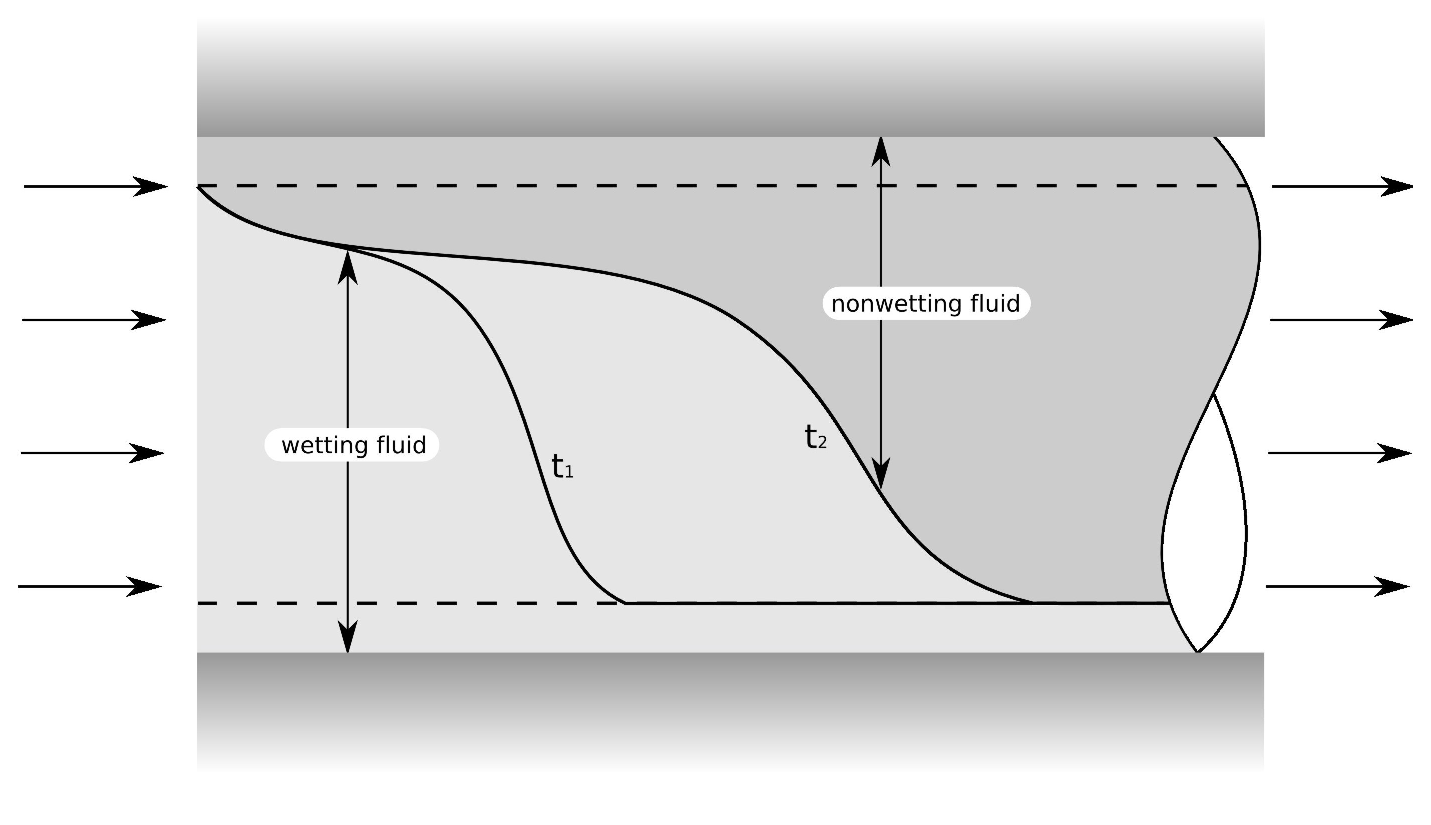
\includegraphics[width=0.7\textwidth]{FLUID_PROPERTIES/figures/egr-scheme.eps}
\captionsetup{format=hang,justification=raggedright,justification=justified}
\caption{Schematic drawing of 1D-two phase flow problem: {\ce{CO2}} is treated as a wetting fluid and displaces the non-wetting methane from the 1D-model domain.}
\label{fig_egr_scheme}
\end{figure}


\subsubsection*{Problem definition}

Initially, a 1D gas reservoir in a depth of $\unit[3500]{m}$ is nearly fully saturated with methane at a pressure of $\mathrm{p_{\ch4}}=\unit[50]{bar}$ and a temperature of $\mathrm{T}=\unit[400]{K}$. The model domain has a length of $\mathrm{L}=\unit[5]{m}$ (see Fig.~\ref{fig_model_setup}). At $\mathrm{x}=\unit[0]{m}$, \co2 with a temperature of $\mathrm{T}=\unit[350]{K}$ is pumped into the aquifer and displaces the residing methane. To show the influence of temperature to fluid properties clearly, the temperature is forced to grow linearly with the distance from the injection point. Time steps at the beginning of the simulation are very short ($\unit[0.1]{s}$), and are growing longer up to $\unit[100]{s}$. Tab.~\ref{tab-h2t-compressible-specs} shows all relevant model specifications.

 \begin{figure}%[h]
\centering
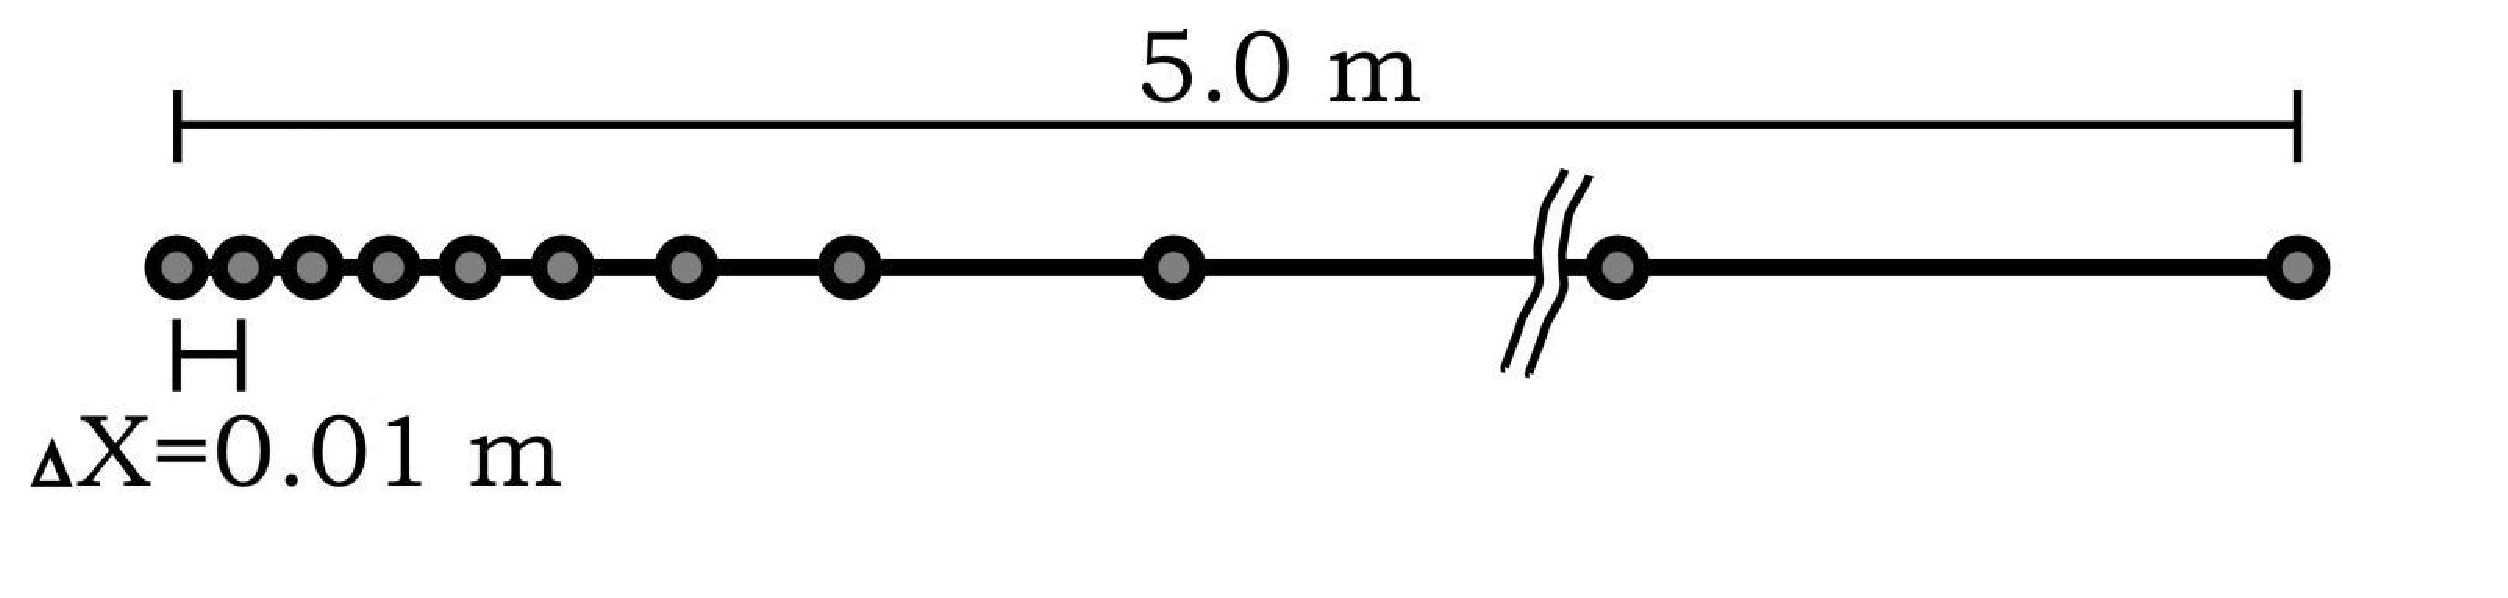
\includegraphics[width=0.7\textwidth]{FLUID_PROPERTIES/figures/modelsetup_h2t_compr.eps}
\captionsetup{format=hang,justification=raggedright,justification=justified}
\caption{Model domain consisting of 1D-line elements with growing lenghts. The length of the first element (at the injectoin point) is 1\,cm.}
\label{fig_model_setup}
\end{figure}


\begin{table}%[ht]
%\centering
%\captionsetup{format=hang,justification=raggedright,justification=justified}
\caption{Parameters used in the H$^2$T-benchmark test example}
\begin{center}
\begin{tabular}{lcr}
\toprule
\textbf{parameter} & \textbf{symbol} & \textbf{value} \\
\midrule
\multicolumn{3}{l}{\textit{spatial discretisation}}\\
\hspace{10pt} element type &  & 1D \\
\hspace{10pt} domain length & L & \unit[5]{m} \\
\hspace{10pt} element number & & 260 \\
\midrule
\multicolumn{3}{l}{\textit{temporal discretisation}}\\
\hspace{10pt} timestep size & $\Delta t$ & \unit[0.1]{s} to \unit[100]{s}\\
\hspace{10pt} timestep number & & \unit[580]{[-]}\\
\hspace{10pt} total time & t & \unit[10\,000]{s}\\
\midrule
\multicolumn{3}{l}{\textit{material properties}}\\
\hspace{10pt} density & $\rho$ & \unit[2500]{kg$\cdot$m$^3$}\\
\midrule
\multicolumn{3}{l}{\textit{\small{\co2} \normalsize{properties}}} \\
\hspace{10pt} density & $\rho(p,T)$ & PREOS \cite{PenRob:75}\\
\hspace{10pt} viscosity & $\eta(\rho,T)$ & \textsc{Fengour} \cite{FenWakVes:98}\\
\hspace{10pt} thermal conductivity & $\lambda$ & -\\
\midrule
\multicolumn{3}{l}{\textit{\small{\ch4} \normalsize{properties}}} \\
\hspace{10pt} density & $\rho(p,T)$ & PREOS \cite{PenRob:75}\\
\hspace{10pt} viscosity & $\eta(\rho,T)$ & \textsc{Friend} \cite{FriElyIng:89}\\
\hspace{10pt} thermal conductivity & $\lambda$ & -\\
\midrule
\multicolumn{3}{l}{\textit{initial conditions}} \\
\hspace{10pt} {\ce{CH4}} saturation & $S_{\ce{CH4}}$ & \unit[0.99]{[-]} \\
\midrule
\multicolumn{3}{l}{\textit{boundary conditions}}\\
\hspace{10pt} {\ce{CH4}} saturation & $S_{\ce{CH4}}$ & \unit[0]{[-]}\\
\hspace{10pt} {\ce{CO2}} pressure & $p_{\ce{CO2}}$ & \unit[5.495]{MPa}\\
\hspace{10pt} temperature left & T & \unit[380]{K}\\
\hspace{10pt} temperature right & T & \unit[420]{K}\\
\multicolumn{3}{c}{\hspace{10pt}(temperature rises linearly from left to right border)} \\
\midrule
\multicolumn{3}{l}{\textit{medium properties}}\\
\hspace{10pt} porosity & $\phi$ & \unit[0.03]{[-]} \\
\hspace{10pt} intrinsic permeability & $\mathbf{K}$ & \unit[$1\cdot 10^{\text{-}12}]{m^2}$ \\
\hspace{10pt} residual {\ce{CO2}} saturation & $S_{r,{\ce{CO2}}}$ & \unit[0.01]{[-]} \\
\hspace{10pt} residual {\ce{CH4}} saturation & $S_{r,{\ce{CH4}}}$ & \unit[0]{[-]} \\
\hspace{10pt} capillary pressure & $p_{c}\left(S_{\operatorname{eff}}\right)$ & Brooks\&Corey  \\
\hspace{10pt} relative permeability & $k_{r}\left(S_{\operatorname{eff}}\right)$ & Brooks\&Corey  \\
\hspace{10pt} soil distribution index & $\lambda$ & \unit[2]{} \\
\hspace{10pt} entry pressure & $p_d$ & \unit[5\,000]{Pa} \\
\bottomrule	
\end{tabular}
\end{center}
\label{tab-h2t-compressible-specs}
\end{table}

% \begin{figure}[ht]
%\centering
%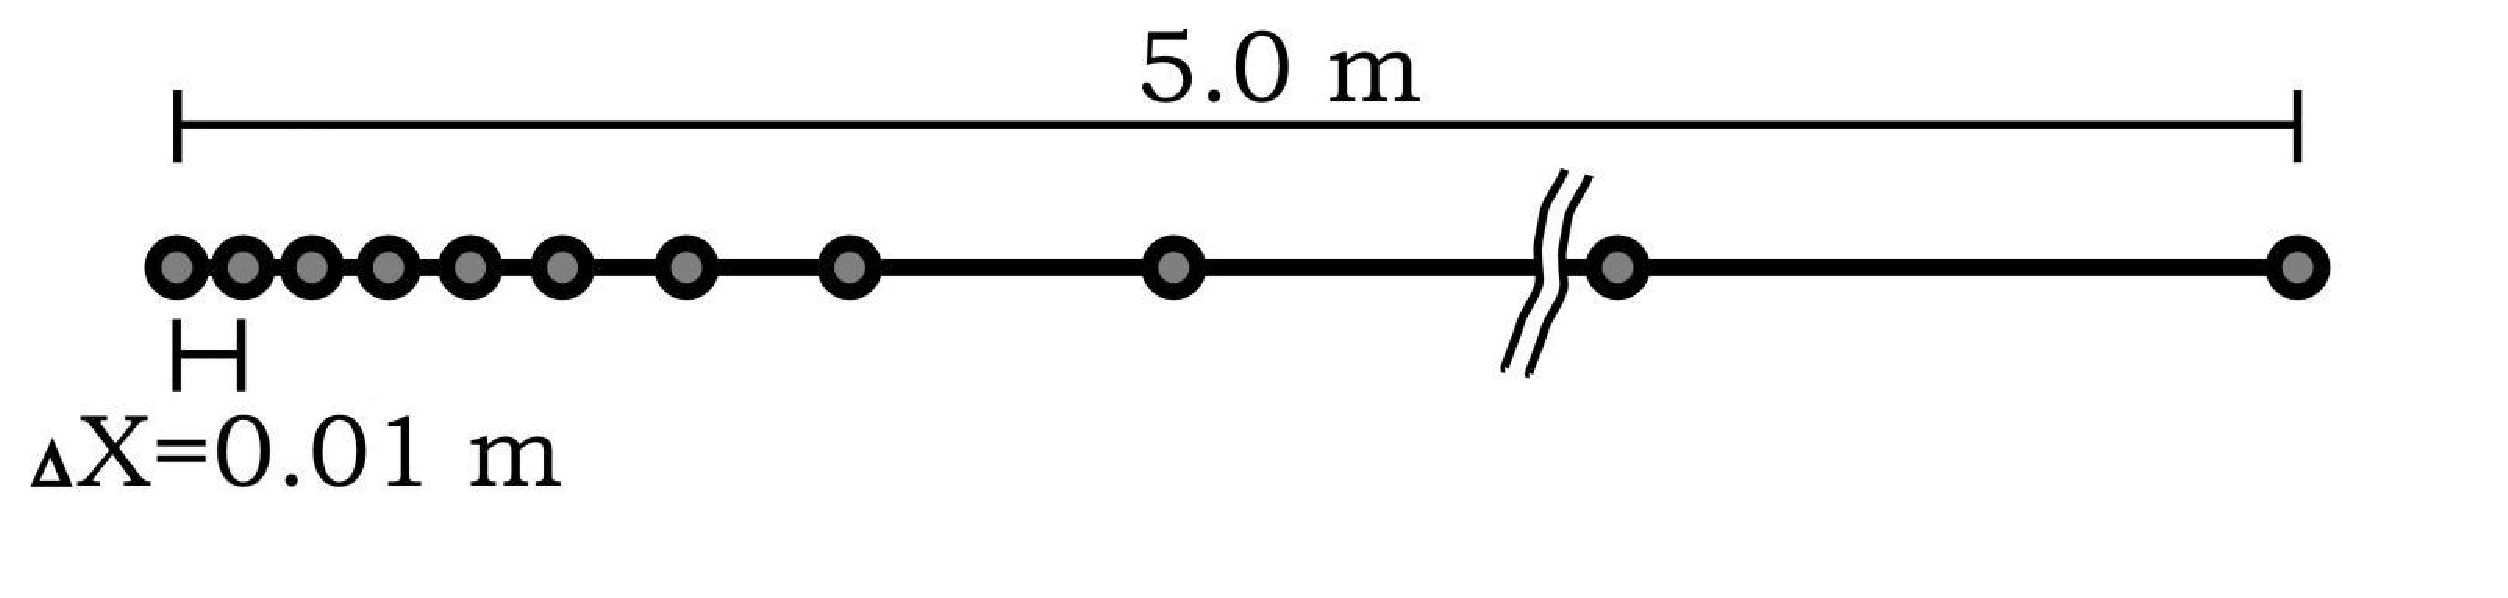
\includegraphics[width=0.7\textwidth]{FLUID_PROPERTIES/figures/modelsetup_h2t_compr.eps}
%\captionsetup{format=hang,justification=raggedright,justification=justified}
%\caption{Model domain consisting of 1D-line elements with growing lenghts. The length of the first element (at the injectoin point) is 1\,cm.}
%\label{fig_model_setup}
%\end{figure}


%%%%%%%%%%%%%%%%%%%%%%%%%%%%%%%%%%%%%%%%%%%%%%%%%%%%%%%%%%%%%%%%%%%%%%%%%%%%%%%%%%%%%%%%%%%%%%%%%%%%%%%%%%%%%%%%%%%%
%\clearpage		%--------->Achtung, eventuell später wieder entfernen

\subsubsection*{Governing equations}

The governing equation for two phase flow in porous media can be written as:

\begin{equation}
\phi\frac{\partial S_\alpha\rho_\alpha}{\partial t} = \operatorname{div}\left(\rho_\alpha\frac{k_{r\alpha}}{\mu_\alpha}\mathbf{K}\left\lbrace\nabla p_\alpha-\rho\mathbf{g}\right\rbrace\right)+\rho_\alpha q_\alpha.
\label{eq_gov_general}
\end{equation}

In the actual test case, no source terms are considered ($\mathrm{q_\alpha}=0$). Since we consider a horizontal 1D-problem, the z coordinate doesn't change, so the gravity term can be necleted as well. We also handle no changes of porosity due to deformation or precipitation, so porosity $\phi$ can be treated as constant. Regarding this assumtions, we can expand \eqref{eq_gov_general} to the following formulation:

\begin{equation}
\phi\frac{\partial S_\alpha}{\partial t}+\phi\frac{S_\alpha}{\rho_\alpha}\left(\frac{\partial\rho_\alpha}{\partial p_\alpha}\frac{\partial p_\alpha}{\partial t}+\frac{\partial\rho_\alpha}{\partial T}\frac{\partial T}{\partial t}\right) = \operatorname{div}\left(\rho_\alpha\frac{k_{r\alpha}\!\left(S_\alpha\right)}{\mu_\alpha\!\left(p_\alpha,T\right)}\mathbf{K}\nabla p_\alpha\right)
\label{eq_gov_specific}
\end{equation}

for both phases $\alpha$. At the present state, density change due to temperature in not considered yet, so

\begin{equation}
\phi\frac{\partial \rho_\alpha}{\partial T}=0,
\label{eq_drho_dT}
\end{equation}

and \eqref{eq_gov_specific} reduces to 

\begin{equation}
\phi\frac{\partial S_\alpha}{\partial t}+\phi\frac{S_\alpha}{\rho_\alpha}\frac{\partial\rho_\alpha}{\partial p_\alpha}\frac{\partial p_\alpha}{\partial t} = \operatorname{div}\left(\rho_\alpha\frac{k_{r\alpha}\!\left(S_\alpha\right)}{\mu_\alpha\!\left(p_\alpha,T\right)}\mathbf{K}\nabla p_\alpha\right).
\label{eq_gov_specific_short}
\end{equation}


The compressibility of fluids due to temperature change will be shown in one of the next benchmarks.

%%%%%%%%%%%%%%%%%%%%%%%%%%%%%%%%%%%%%%%%%%%%%%%%%%%%%%%%%%%%%%%%%%%%%%%%%%%%%%%%%%%%%%%%%%%%%%%%%%%%%%%%%%%%%%%%%%%%
\subsubsection*{Constitutive equations}

A general equation of state for pure substances by \textsc{Peng\&Robinson} \cite{PenRob:75} was chosen to determine the densities of carbon dioxide and methane. The viscosity of both fluids is computed by correlations from Fenghour et al. \cite{FenWakVes:98} for {\ce{CO2}} and Friend et al. \cite{FriElyIng:89} for {\ce{CH4}}. Both density and viscosity correlations depend on pressure and temperature conditions and are described in detail in sections \ref{eos-density} and \ref{sec-viscosity}.

%%%%%%%%%%%%%%%%%%%%%%%%%%%%%%%%%%%%%%%%%%%%%%%%%%%%%%%%%%%%%%%%%%%%%%%%%%%%%%%%%%%%%%%%%%%%%%%%%%%%%%%%%%%%%%%%%%%%
\subsubsection*{Results}

The functionality of the fluid property functions can be evaluated by comparing the simulation results with constant fluid property models...
In comparison with the H2T-McWhorter problem (\ref{MWPIsoTwoPhaseFlow}), the plume of the wetting fluid ...

%\begin{figure}[h]
%\centering
%\includegraphics[width=0.6\textwidth]{figures/AA_6.eps}
%\captionsetup{format=hang,justification=raggedright,justification=justified}
%\caption{Saturation distribution of CO2 and H2O at time. A better looking result plot is coming soon...}
%\label{AA_6_pic}
%\end{figure}



\begin{table}[h]
%\centering
%\captionsetup{format=hang,justification=raggedright,justification=justified}
\caption{Benchmark deposit}
\begin{center}
\begin{tabular}{lll}
\toprule
Deposit & Version & Date \\
\midrule
\texttt{GROUNDWATER\_FLOW$\backslash$EOS$\backslash$H2T}& 4.10.02 & Oct. 2009 \\
\bottomrule
\end{tabular}
\end{center}
\end{table}
